\begin{figure}
    \centering
    \subfloat[Permuted spectral densities]{%
        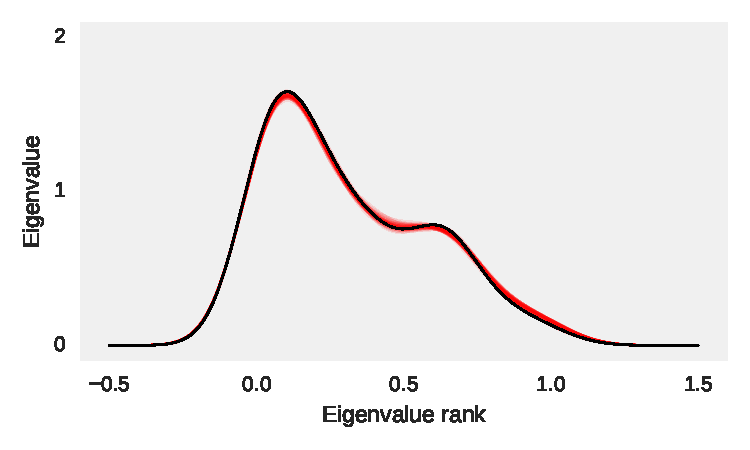
\includegraphics[width=0.5\textwidth]{figures/gopher_louse_spectral_density_permutations}
    }
    \subfloat[Shannon-Jensen distances]{%
        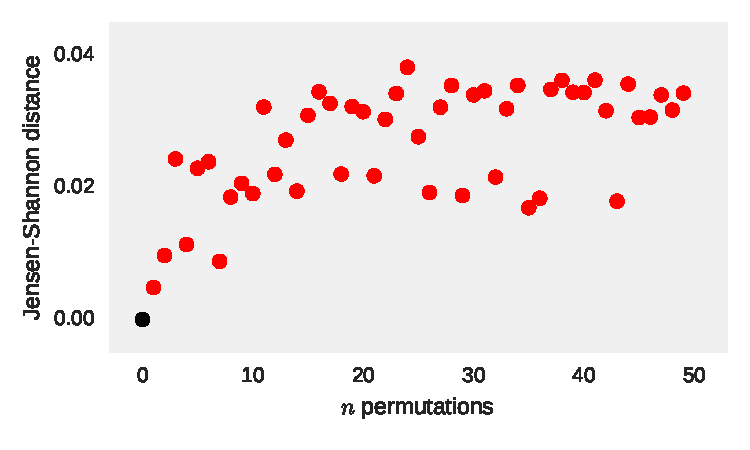
\includegraphics[width=0.5\textwidth]{figures/gopher_louse_spectral_density_permutation_distances}
    }
    \caption{Spectral density distributions of successively permuted interactions among pocket gophers and their chewing lice parasites from Hafner {\em et al.} \cite{hafner1994disparate} \textbf{(a)} and the Shannon-Jensen distances between each with respect to the spectral density distribution of the un-permuted interaction \textbf{(b)}.}
    \label{fig:FP_permuted_distances}
\end{figure}